   
        
        \begin{ledgroupsized}[r]{120mm}
        \footnotesize 
        \pstart        
        \noindent\textbf{\"{U}berlieferung:}  
        \pend
        \end{ledgroupsized}
      
       
              \begin{ledgroupsized}[r]{114mm}
              \footnotesize 
              \pstart \parindent -6mm
              \makebox[6mm][l]{\textit{L}}Konzept: LH XXXVIII Bl. 19\textendash20. 1 Bog. 4\textsuperscript{o}. Gesamtumfang 2 S. Textfolge: Bl. 19 r\textsuperscript{o}, Bl. 20 v\textsuperscript{o} unten, Bl. 19 v\textsuperscript{o} ober- und unterhalb einer Zeichnung, die zu N. 13\protect\raisebox{-0.5ex}{\tiny{1}} geh\"{o}rt. Die Zeichnung unseres St\"{u}ckes in der Mitte von Bl. 19 r\textsuperscript{o}. Die \"{u}brigen Seiten N. 13\protect\raisebox{-0.5ex}{\tiny{1}} und N. 13\protect\raisebox{-0.5ex}{\tiny{2}}. Zur Anordnung der drei St\"{u}cke auf dem Bogen vgl. die \"{U}berlieferung zu N. 13\protect\raisebox{-0.5ex}{\tiny{1}}. \pend
              \end{ledgroupsized}
       
              \begin{ledgroupsized}[r]{114mm}
              \footnotesize 
              \pstart \parindent -6mm
              \makebox[6mm][l]{\textit{E}}\cite{00243}\textsc{Gerland} 1906, S.~199\textendash200.\\Cc 2, Nr. 477 tlw. \pend
              \end{ledgroupsized}
        \vspace*{8mm}
        \pstart 
        \normalsize
      [19 r\textsuperscript{o}] \edtext{Observata inclinatione determinari potest latitudo loci.}{\lemma{}\Afootnote{ \textit{ (1) }\ Observata mutatione inclinationis\protect\index{Sachverzeichnis}{inclinatio|textit} loci \textit{ (2) }\ Si in diversis locis inclinatio\protect\index{Sachverzeichnis}{inclinatio|textit} observetur successive cognitaque sit eorum duorum locorum distantia, dabitur meridianus\protect\index{Sachverzeichnis}{meridianus|textit} loci et latitudo\protect\index{Sachverzeichnis}{latitudo|textit} utriusque \textit{ (3) }\ Observata [...] loci. \textit{ L}}} Cognita duorum locorum latitudine\protect\index{Sachverzeichnis}{latitudo}, et distantia cognita erit longitudinum\protect\index{Sachverzeichnis}{longitudo} differentia.\pend \pstart Determinare: mutatio acus\protect\index{Sachverzeichnis}{acus!magnetica}, sitne ab acu\protect\index{Sachverzeichnis}{acus!magnetica}, an a navi\protect\index{Sachverzeichnis}{navis}.\pend
         \begin{center}
         %\begin{wrapfigure}{l}{0.6\textwidth}          
         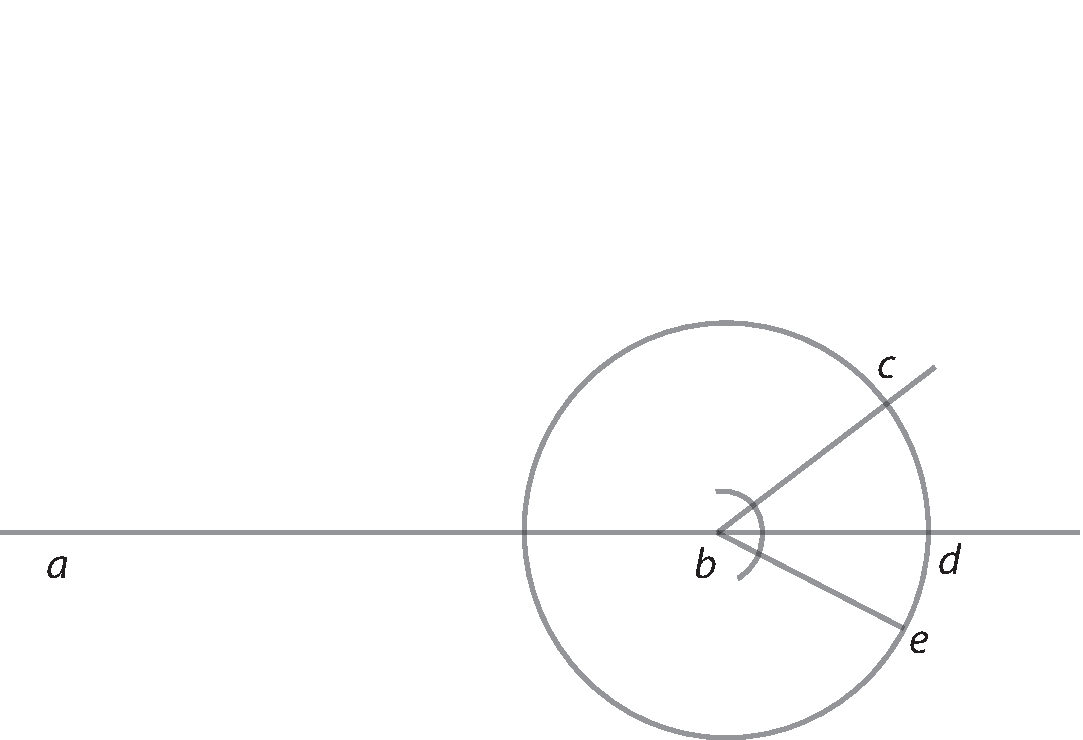
\includegraphics[width=0.6\textwidth]{images/38_19r}\\
         %\caption{Bildbeschreibung}
         \textit{[Fig. 1, tlw. Blindzeichnung]}
         %\end{wrapfigure}
         \end{center}
      \pstart Duo sunt casus. Cursus scilicet navis\protect\index{Sachverzeichnis}{navis} vel ita comparatus est, ut semper declinet nunc quidem \edtext{per satis longum temporis spatium a septentrione in orientem ab Austro in occidentem, vel ut a septentrione in occidentem ab Austro in orientem.}{\lemma{quidem}\Afootnote{ \textit{ (1) }\ ab Austro in orientem \textit{ (2) }\ per [...] orientem. \textit{ L}}} Similiter acus\protect\index{Sachverzeichnis}{acus!magnetica} nunc per satis longum spatium declinat aut in orientem tantum aut in occidentem tantum, scilicet a septentrione. Supponamus ergo primo navem\protect\index{Sachverzeichnis}{navis} et acum\protect\index{Sachverzeichnis}{acus!magnetica} declinare eodem, scilicet \edtext{a septentrione}{\lemma{scilicet}\Afootnote{ \textit{ (1) }\ ab Austro \textit{ (2) }\ a septentrione \textit{ L}}} v.g. in orientem aut contra. Ponatur linea cursus navis\protect\index{Sachverzeichnis}{navis} esse \textit{ab}[,] septentrio \textit{a}[,] navis\protect\index{Sachverzeichnis}{navis} declinet in orientem ut linea cursus fiat \textit{bc} si acus\protect\index{Sachverzeichnis}{acus!magnetica} \textit{bd} supponatur immobilis, manifestum est eam in circulo immobiliter ad \textit{bc} affixo, centro \textit{b} designaturam esse arcum flexus \textit{cd}. Ponatur interea acus\protect\index{Sachverzeichnis}{acus!magnetica} itidem declinare versus orientem seu versus \textit{c} manifestum est si acus\protect\index{Sachverzeichnis}{acus!magnetica} spectetur ut immobilis, uti certe in navi\protect\index{Sachverzeichnis}{navis} spectanda est, in effectu lineam cursus \textit{bc} retroactam versus \textit{d}. Et proinde inclinationem\protect\index{Sachverzeichnis}{inclinatio} navis\protect\index{Sachverzeichnis}{navis} et acus\protect\index{Sachverzeichnis}{acus!magnetica} in eandem plagam quoad effectum motus in Tabula seu pyxide\protect\index{Sachverzeichnis}{pyxis} designandi, esse sibi contrarias.\footnote{\textit{Links daneben:} Faciendum ut omnia sint difficilis motus, sed fortificanda acus\protect\index{Sachverzeichnis}{acus!magnetica}. } Ut ergo determinetur in Tabula quando et quatenus \edtext{mutuo situ Tabulae fuerit}{\lemma{quatenus}\Afootnote{ \textit{ (1) }\ motus sit \textit{ (2) }\ mutuo situ Tabulae fuerit \textit{ L}}} a \textit{d} versus \textit{c} id est a navi\protect\index{Sachverzeichnis}{navis} vel a \textit{c} versus \textit{d} id est ab acu\protect\index{Sachverzeichnis}{acus!magnetica}: ita fieri potest, sit annulus \textit{cd} in circulo \textit{cd} mobilis, divisus in gradus etc. non minus quam circulus. Is annulus ita comparatus sit, ut quando ab acu\protect\index{Sachverzeichnis}{acus!magnetica} premitur versus \textit{d} quod fit cum acus\protect\index{Sachverzeichnis}{acus!magnetica} tendit versus \textit{d} id est cum navis\protect\index{Sachverzeichnis}{navis} sola versus \textit{c} seu declinat, tunc non possit a circulo separari, ac proinde invita acu\protect\index{Sachverzeichnis}{acus!magnetica} abripiatur \edtext{a circulo}{\lemma{}\Afootnote{a circulo \textit{ erg.} \textit{ L}}}. Contra quando ab acu\protect\index{Sachverzeichnis}{acus!magnetica} premitur versus \textit{c} id est cum acus \protect\index{Sachverzeichnis}{acus!magnetica} declinat abripiatur cum acu\protect\index{Sachverzeichnis}{acus!magnetica} relicto circulo, ita annulus monstrabit flexus navis\protect\index{Sachverzeichnis}{navis} sine declinatione\protect\index{Sachverzeichnis}{declinatio} acus\protect\index{Sachverzeichnis}{acus!magnetica}.